\chapter{Metode}
\section{Proiectarea și Implementarea Arhitecturii Hardware}

	Pentru implementarea conceptului de Edge Computing, sistemul trebuie să poată îndeplini gestionarea concomitentă a achiziției de date în timp real, preprocesarea acestora prin algoritmul de învățare automată și comunicarea rezultatelor. Astfel am optat pentru microcontrolerul ESP32 având un procesor dual-core și resurse de memorie minime adecvate pentru rularea modelelor de Machine Learning la nivel local. \cite{esp32_datasheet}
	Pentru a colecta datele am construit un stand experimental. Ansamblul este alcătuit dintr-un motor de curent continuu (DC) cu reductor tip TT, echipat cu o roată din material de plastic/cauciuc. Acesta este alimentat de o sursă externă din 4 baterii de tip AA. Controlul turației motorului s-a realizat prin intermediul unui modul driver L298N (punte H). \cite{handson:l298n_module}
	Pentru achiziția semnalelor de vibrație s-a folosit senzorul inerțial MPU6050, fixat rigid pe carcasa de plastic a motorului. Senzorul comunică cu microcontrolerul ESP32 prin intermediul protocolului bidirecțional I2C. \cite{nxp:i2c_specification}
	\begin{figure}[htbp]
		\centering
		\begin{tikzpicture}[
			node distance=2cm and 2.5cm,
			block/.style={rectangle, draw, fill=gray!10, text width=3cm, align=center, minimum height=1.2cm, font=\small\sffamily, thick},
			sensor/.style={rectangle, draw, fill=cyan!10, text width=3cm, align=center, minimum height=1.2cm, font=\small\sffamily, thick},
			power/.style={rectangle, draw, fill=orange!10, text width=2.5cm, align=center, minimum height=1.2cm, font=\small\sffamily, thick},
			ui/.style={rectangle, draw, fill=magenta!10, text width=3cm, align=center, minimum height=1.2cm, rounded corners, font=\small\sffamily, thick},
			arrow/.style={-{Stealth[scale=1.2]}, thick},
			dashed_arrow/.style={-{Stealth[scale=1.2]}, thick, dashed}
			]
			
			% 1. Plasarea nodurilor într-o grilă logică
			\node (driver) [block] {Driver Motor\\L298N};
			\node (motor) [block, right=of driver] {Motor CC (TT)};
			\node (mpu) [sensor, below=of motor] {MPU6050\\(Accel/Giro)};
			\node (esp32) [block, below=of driver] {ESP32\\(Edge Inference)};
			\node (power) [power, left=of driver] {Sursă 4xAA};
			\node (web) [ui, below=of esp32] {Interfață Web / PC};
			
			% 2. Trasarea liniilor (conexiuni de putere și semnal)
			% Alimentare către driver (linie dreaptă)
			\draw [arrow] (power) -- node[above, font=\footnotesize] {Vin/GND} (driver);
			
			% Alimentare către ESP32 (rutare ortogonală 90 grade - corectată)
			\draw [arrow] (power) |- node[above, near end, font=\footnotesize] {5V/GND} (esp32);
			
			% Control driver -> motor
			\draw [arrow] (driver) -- node[above, font=\footnotesize] {Tensiune} (motor);
			
			% Comandă ESP32 -> driver
			\draw [arrow] (esp32) -- node[right, font=\footnotesize] {PWM (Viteză)} (driver);
			
			% Cuplaj mecanic Motor -> MPU (linie punctată)
			\draw [dashed_arrow] (motor) -- node[right, font=\footnotesize] {Montaj rigid} (mpu);
			
			% Date MPU -> ESP32
			\draw [arrow] (mpu) -- node[above, font=\footnotesize] {I2C (SDA/SCL)} (esp32);
			
			% Monitorizare ESP32 -> Web
			\draw [arrow] (esp32) -- node[right, font=\footnotesize] {HTTP / WiFi} (web);
			
		\end{tikzpicture}
		\caption{Diagrama bloc a arhitecturii hardware și fluxul de semnale. ESP32 centralizează achiziția, inferența și comunicarea, eliminând necesitatea procesării externe.}
		\label{fig:diagrama_bloc_rafinata}
	\end{figure}
	\begin{figure}[htbp]
		\centering
		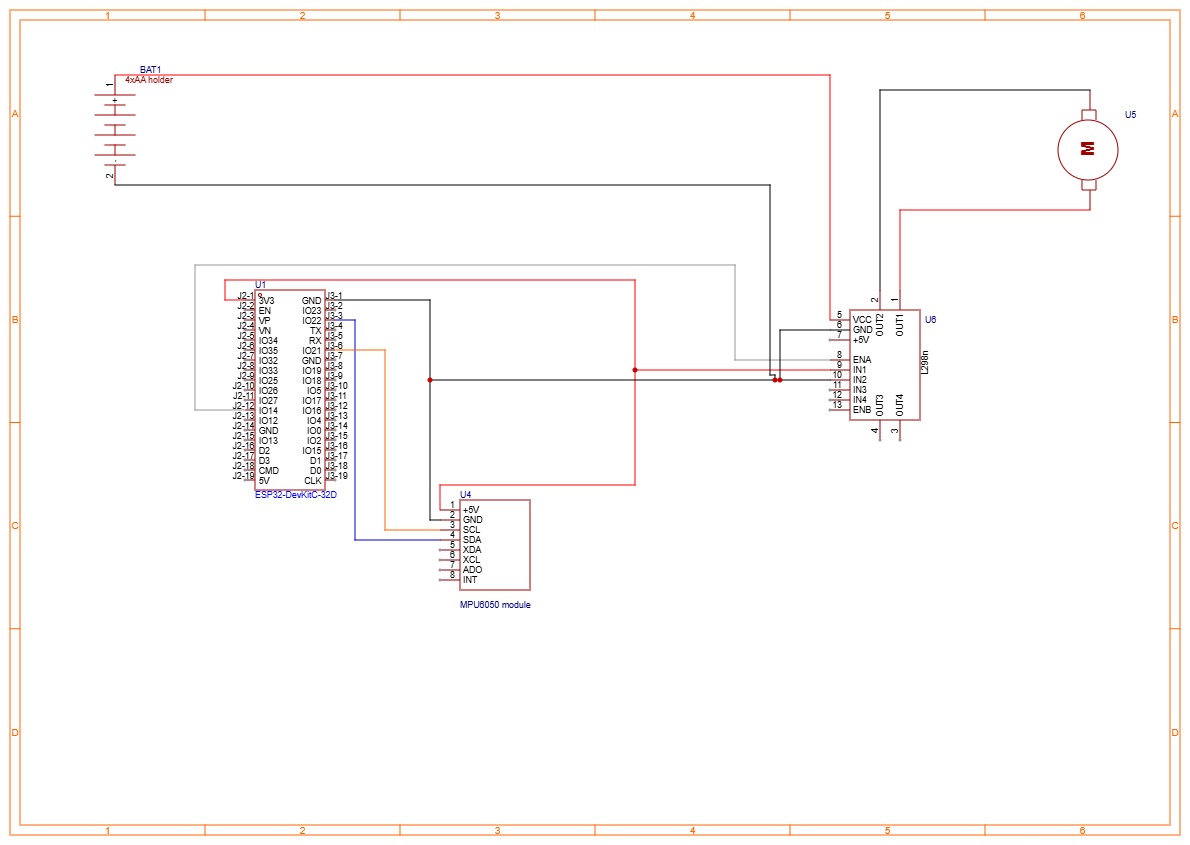
\includegraphics[width=0.7\textwidth]{Schema_Electrica.png} 
		\caption{Diagramă electrică realizată folosind mediul de dezvoltare asistat de calculator EasyEDA}
		\label{fig:schema_electrica}
	\end{figure}
	
	Din punct de vedere software, am utilizat mediul de dezvoltare Arduino pentru ESP împreună cu biblioteca standard Wire.h. \cite{arduino:wire} Pinii microcontrolerului ESP32 pe care i-am folosit pentru această comunicare sunt GPIO 21 pentru semnalul de date și GPIO 22 pentru semnalul de ceas. \cite{esp32_datasheet} Iar pentru abstractizarea citirii și scrierii regiștrilor interni ai senzorului am folosit biblioteca Adafruit\_MPU6050 \cite{adafruit:mpu6050}, împreună cu dependențele Adafruit\_Sensor si Adafruit\_BusIO. \cite{adafruit:sensor, adafruit:busio} Aceste biblioteci realizează extragerea valorilor brute și convertirea lor în unități fizice standard, precum $\frac{m}{s^2}$ pentru accelerație și $\frac{rad}{s}$ pentru viteza unghiulară.
	
\subsection{Configurarea Senzorului și Controlul Motorului}
	
	Am modificat parametrii senzorului calibrându-i corect pentru semnătura vibrațională a defectelor mecanice. Așadar am extins gama de măsurare a accelerometrului la $\pm 16$ prin „MPU6050\_RANGE\_16\_G” conform documentației pentru a preveni saturarea semnalului la șocurile mecanice joase. Totodată am setat gama giroscopului la $\pm 500^\circ/s$ prin „MPU6050\_RANGE\_500\_DEG” pentru a asigura un echilibru optim între rezoluție și capacitatea de captare a mișcării de rotație. Iar pentru atenuarea zgomotului mecanic de înaltă frecvența am activat filtrul trece-jos digital intern al senzorului MPU6050, cu o frecvență de tăiere setată la 21 HZ prin „MPU6050\_BAND\_21\_HZ”. \cite{invensense:mpu6050_datasheet}
	
	Controlul motorului este realizat prin generarea unui semnal PWM aplicat pe pinul de enable ENA al driverului de motor conectat la GPIO 14. Modulul PWM intern al ESP32 are o configurație ce utilizează frecvența de 5000 Hz și o rezoluție de 8 biți, astfel permite setarea precisă a turației prin comanda „TARGET\_PWM = 255” care corespunde funcționării la capacitatea setată pe durata colectării seturilor de date. \cite{esp32_datasheet}

\section{Achiziția Datelor și Construcția Setului de Date}
\subsection{Abordarea Secvențială vs. Tabulară cu Lagging} \label{subsec:abordare_secventiala}
	
	Furnizarea datelor în flux continuu al senzorului \cite{esp32_datasheet} m-a obligat să preprocesez datele înainte de a le introduce în algoritmul de machine learning. În faza de cercetare am analizat diferența dintre abordarea tabulară clasică bazată pe lagging și abordarea secvențială reprezentată de fereastra glisantă.
	În abordarea tabulară tradițională cu tehnica de lagging istoricul senzorului este aplatizat pe un singur rând de date.  Deși această metodă este frecvent folosită în algoritmii clasici, prezintă dezavantaje majore precum: acela de distrugere a ierarhiei spațio-temporale a semnalului, generarea unui spațiu al caracteristicilor extrem de mare și nu prezintă invarianță la translație. Din acest motiv o vibrație care apare la începutul eșantionului va fi tratată complet diferit de aceeași vibrație apărută la finalul acestuia.
	Astfel am optat pentru o abordare secvențială. Tehnica secvențială păstrează formatul bidimensional al datelor, permițând astfel rețelei convoluționale 1D să aplice filtre de-a lungul axei temporale pentru detecția tiparelor de oscilație. \cite{invensense:mpu6050_datasheet} Am ales dimensiunea ferestrei de 128 de eșantioane \cite{ince2016real} deoarece frecvența de eșantionare este de 100 Hz \cite{alfarag3embedded}, astfel acopăr 1,28 secunde, fiind un interval suficient pentru capturarea unui ciclu complet de vibrație mecanică. Pasul de 64 de eșantionare de suprapunere, fiind unul de 50\%, reprezintă un standard în procesarea semnalelor temporale. \cite{gupta2025embedded, kolok2025low} Astfel, sistemul necesită minimum 128 de eșantioane, echivalentul a 1,28 secunde de achiziție, pentru a genera prima predicție, iar datorită suprapunerii de 50\% predicțiile ulterioare sunt produse la fiecare 0,64 secunde.
	
\subsection{Definirea Claselor și Fluxul de Procesare}
	
	Microcontrolerul a fost programat să citească date de pe cele 6 axe, 3 pentru accelerație și 3 pentru giroscop, la o frecvență de eșantionare prestabilită. Valorile citite, împreună cu semnalul PWM aplicat driverului L298N \cite{handson:l298n_module} pentru comanda vitezei, au fost transmise și salvate într-un fișier local pentru a forma setul de date inițial.
	Pentru a antrena rețeaua 1D CNN să recunoască corect diferite stări de funcționare și defecte incipiente, au fost simulate fizic, în mod controlat, următoarele 5 scenarii:
	\begin{tcolorbox}[
		colback=orange!20!white,
		colframe=orange!80!black,
		boxsep=2pt,
		left=4pt, right=4pt,
		top=3pt, bottom=3pt
		]
		\begin{itemize}[noitemsep, topsep=2pt]
			\item \textbf{Clasa 0 (Repaus):} Motorul oprit, calibrează algoritmul pe zgomotul de fond și vibrațiile ambientale.
			\item \textbf{Clasa 1 (Normal):} Ansamblul rulează la parametri nominali, fără perturbații mecanice.
			\item \textbf{Clasa 2 (Dezechilibru):} Simetria roții alterată intenționat, generând vibrații specifice rotoarelor dezechilibrate.
			\item \textbf{Clasa 3 (Frecare):} Forță de frecare externă aplicată asupra roții în mișcare.
			\item \textbf{Clasa 4 (Fixare deficitară):} Sistem de prindere slăbit, simulând joc mecanic și trepidații (Figura~\ref{fig:clase_defecte}).
		\end{itemize}
	\end{tcolorbox}

	\begin{figure}[htbp]
		\centering
		\begin{minipage}[b]{0.3\textwidth} \centering 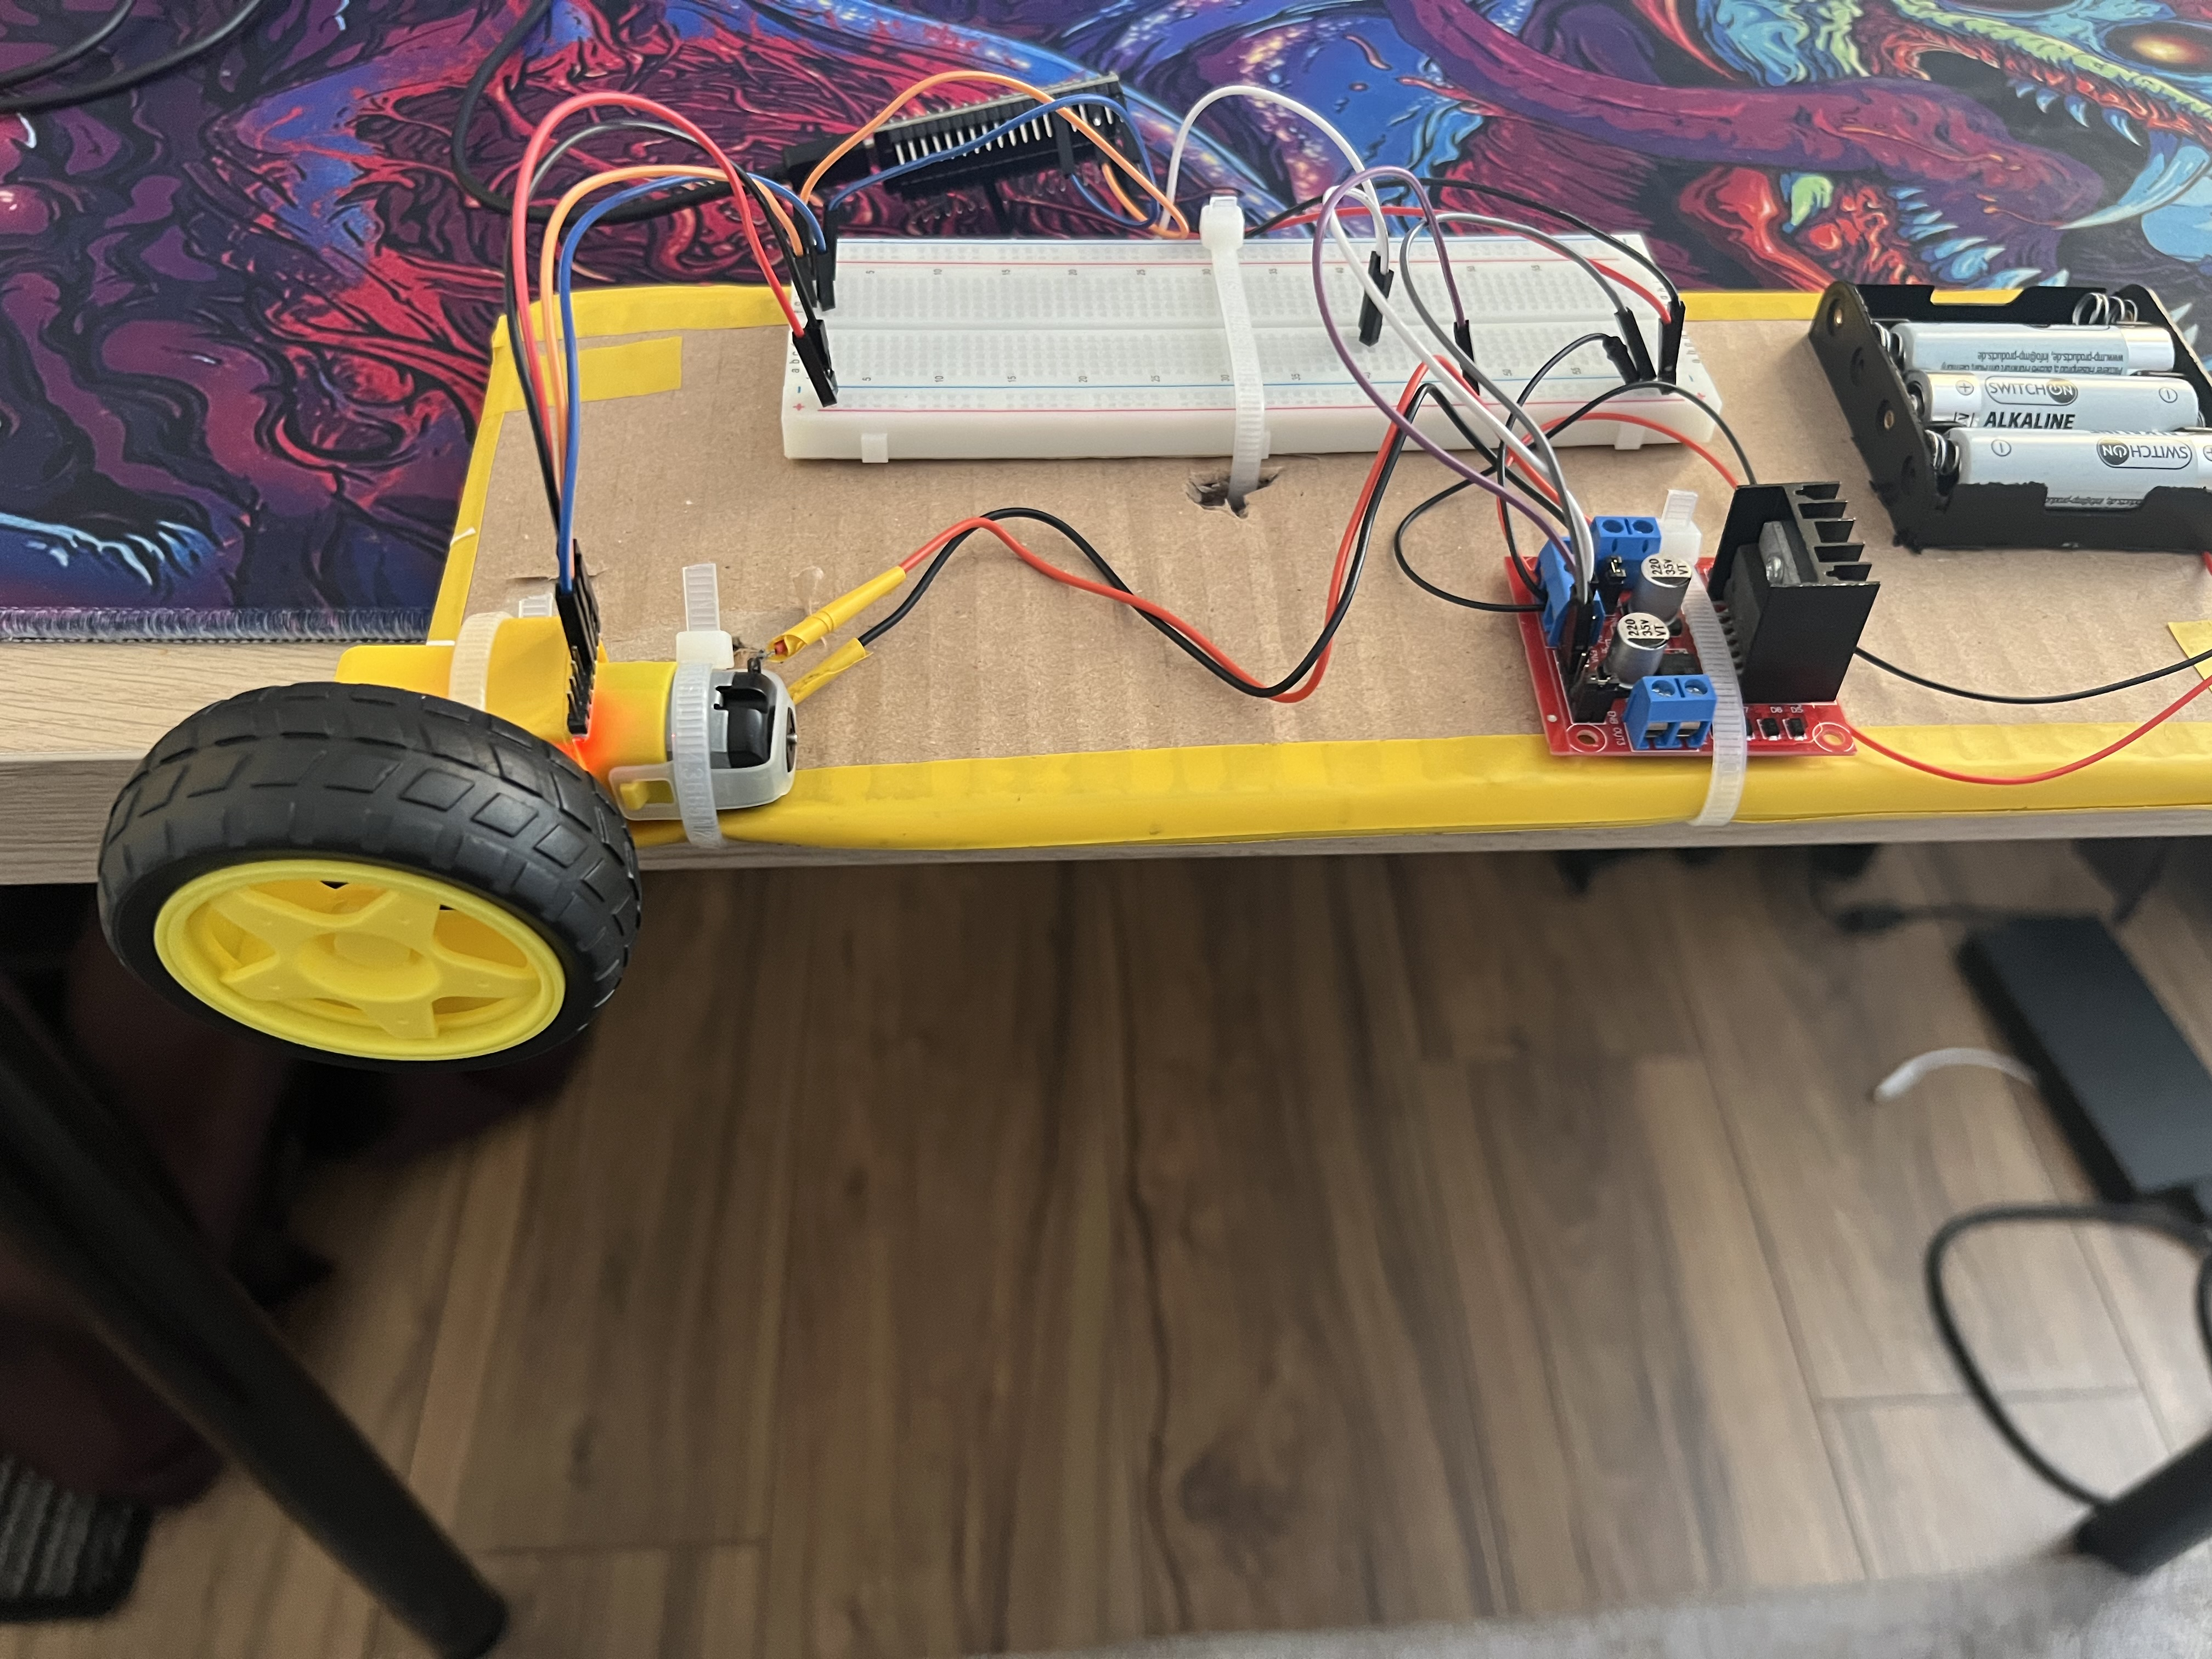
\includegraphics[width=\textwidth]{Montaj_normal.jpeg} \caption*{a) Normal / Repaus} \end{minipage}
		\hfill
		\begin{minipage}[b]{0.3\textwidth} \centering 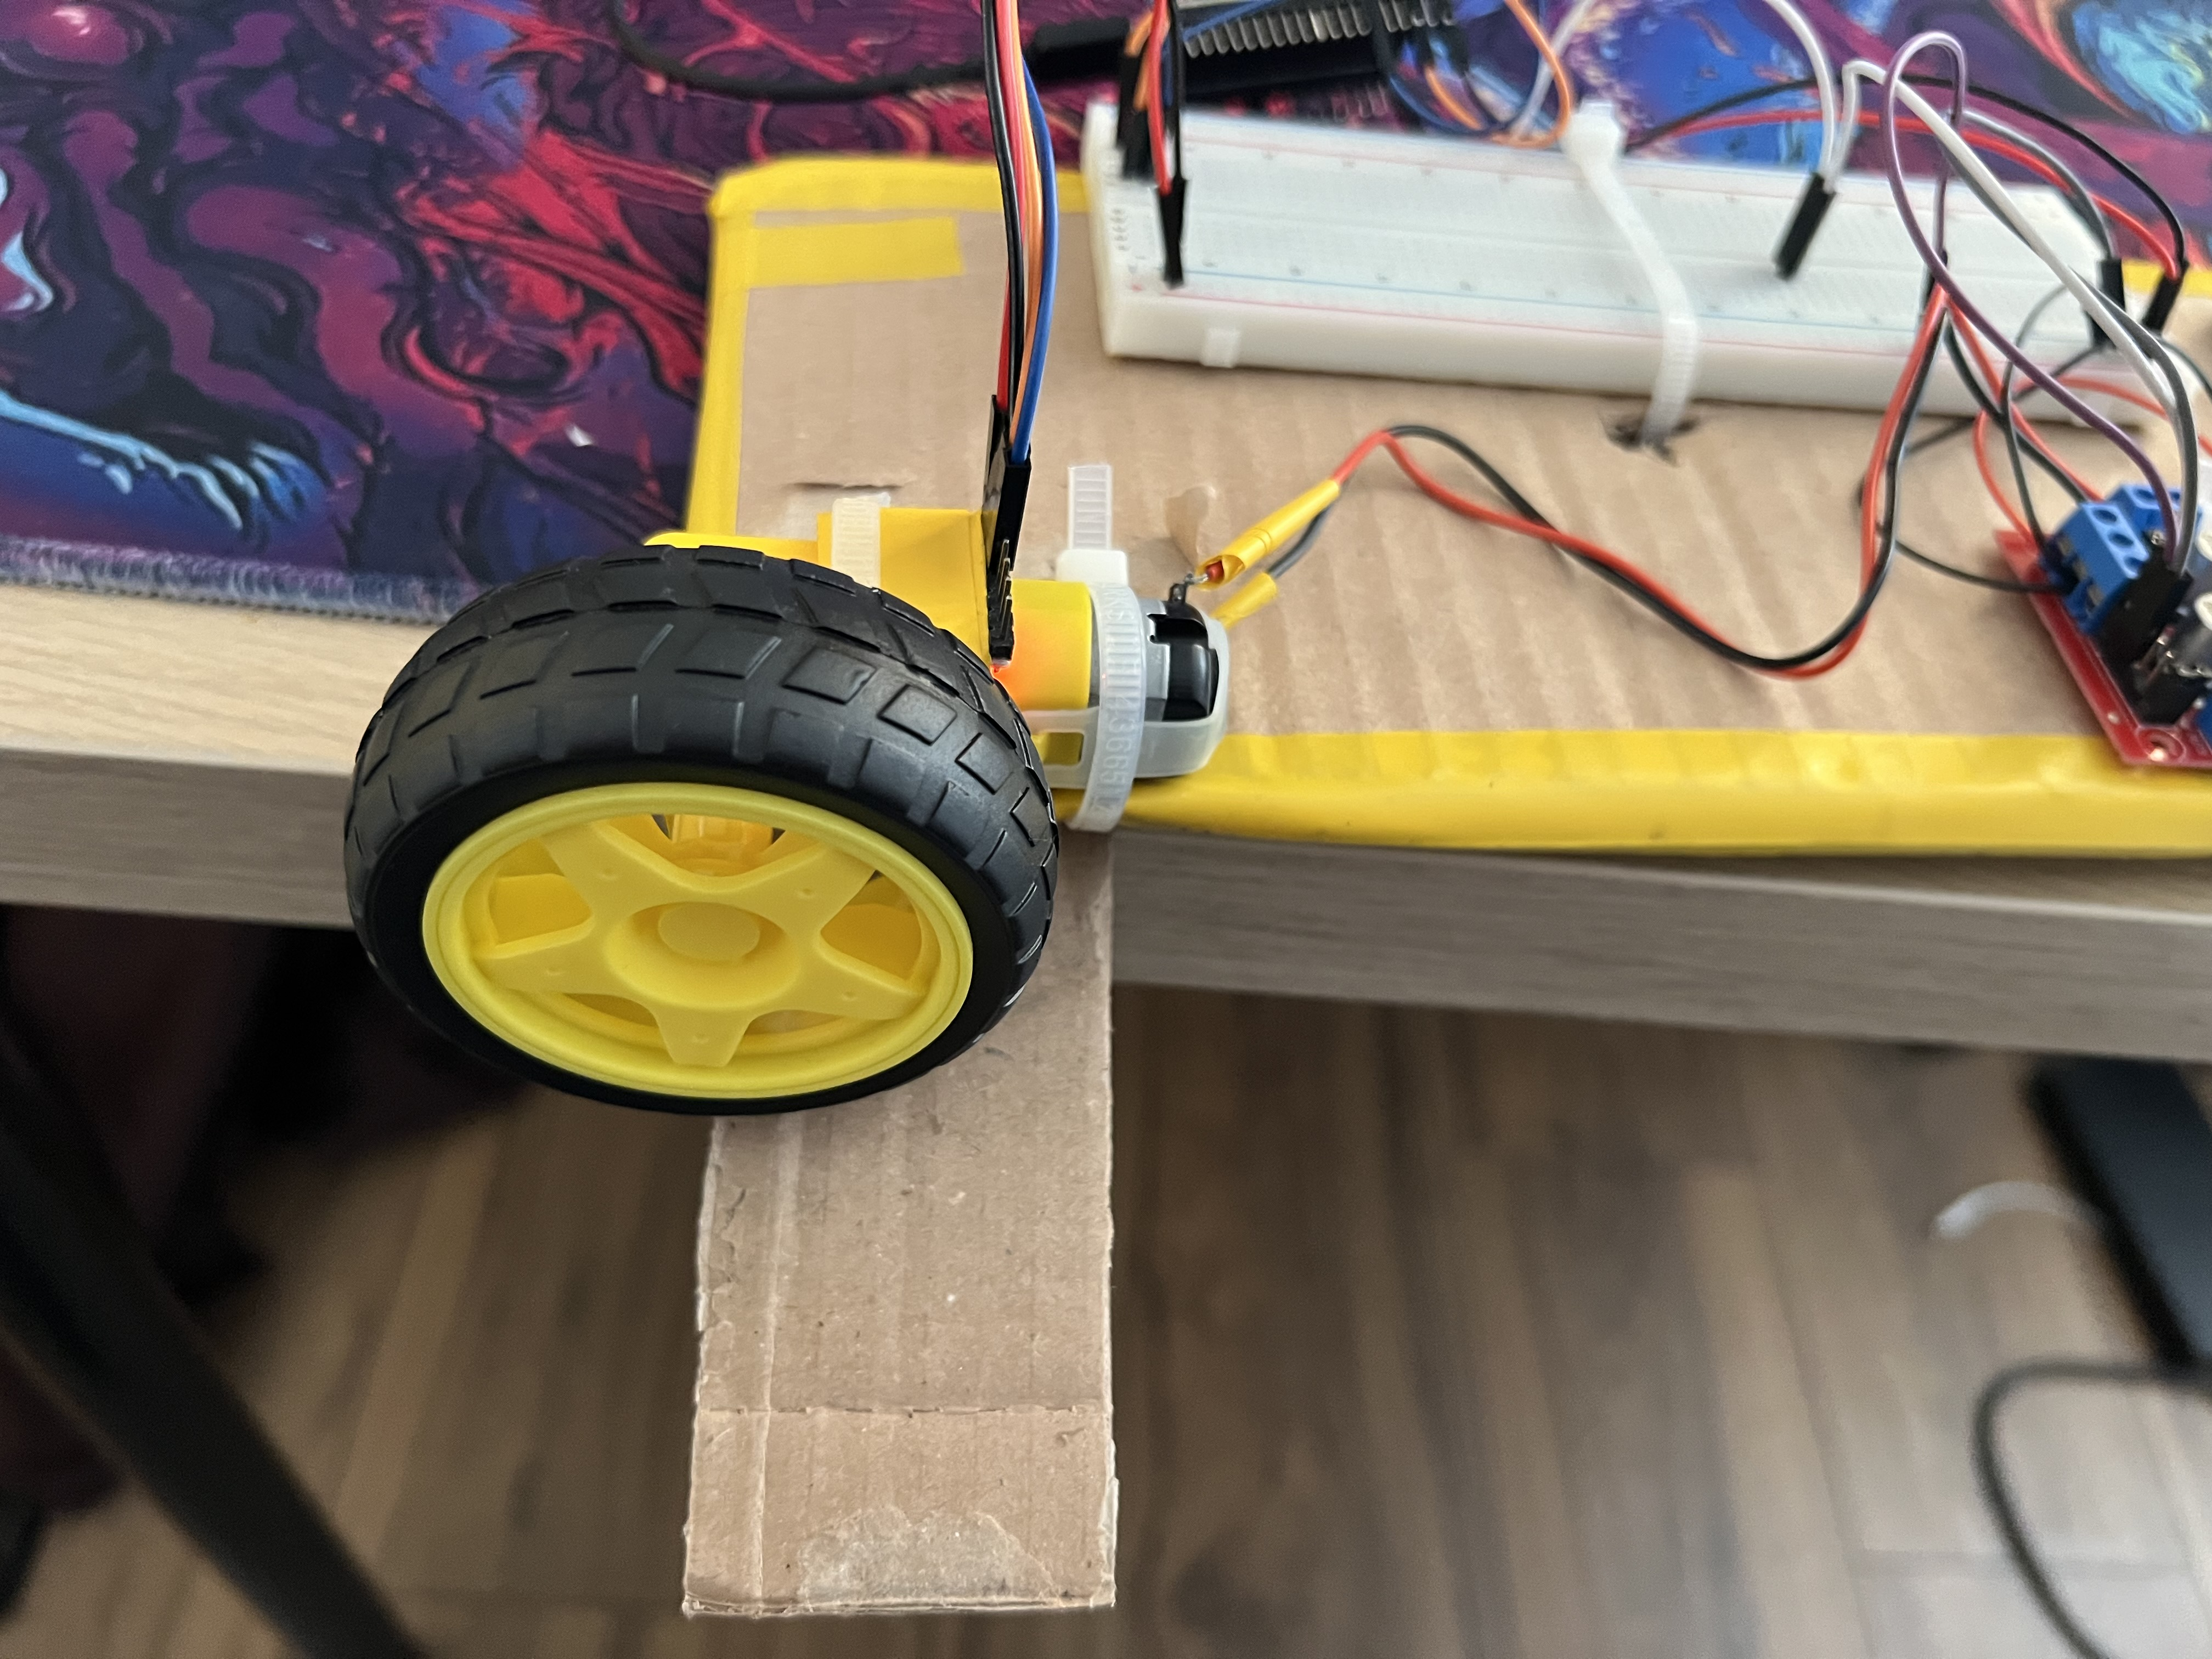
\includegraphics[width=\textwidth]{Frecare.jpeg} \caption*{b) Frecare indusă} \end{minipage}
		\hfill
		\begin{minipage}[b]{0.3\textwidth} \centering 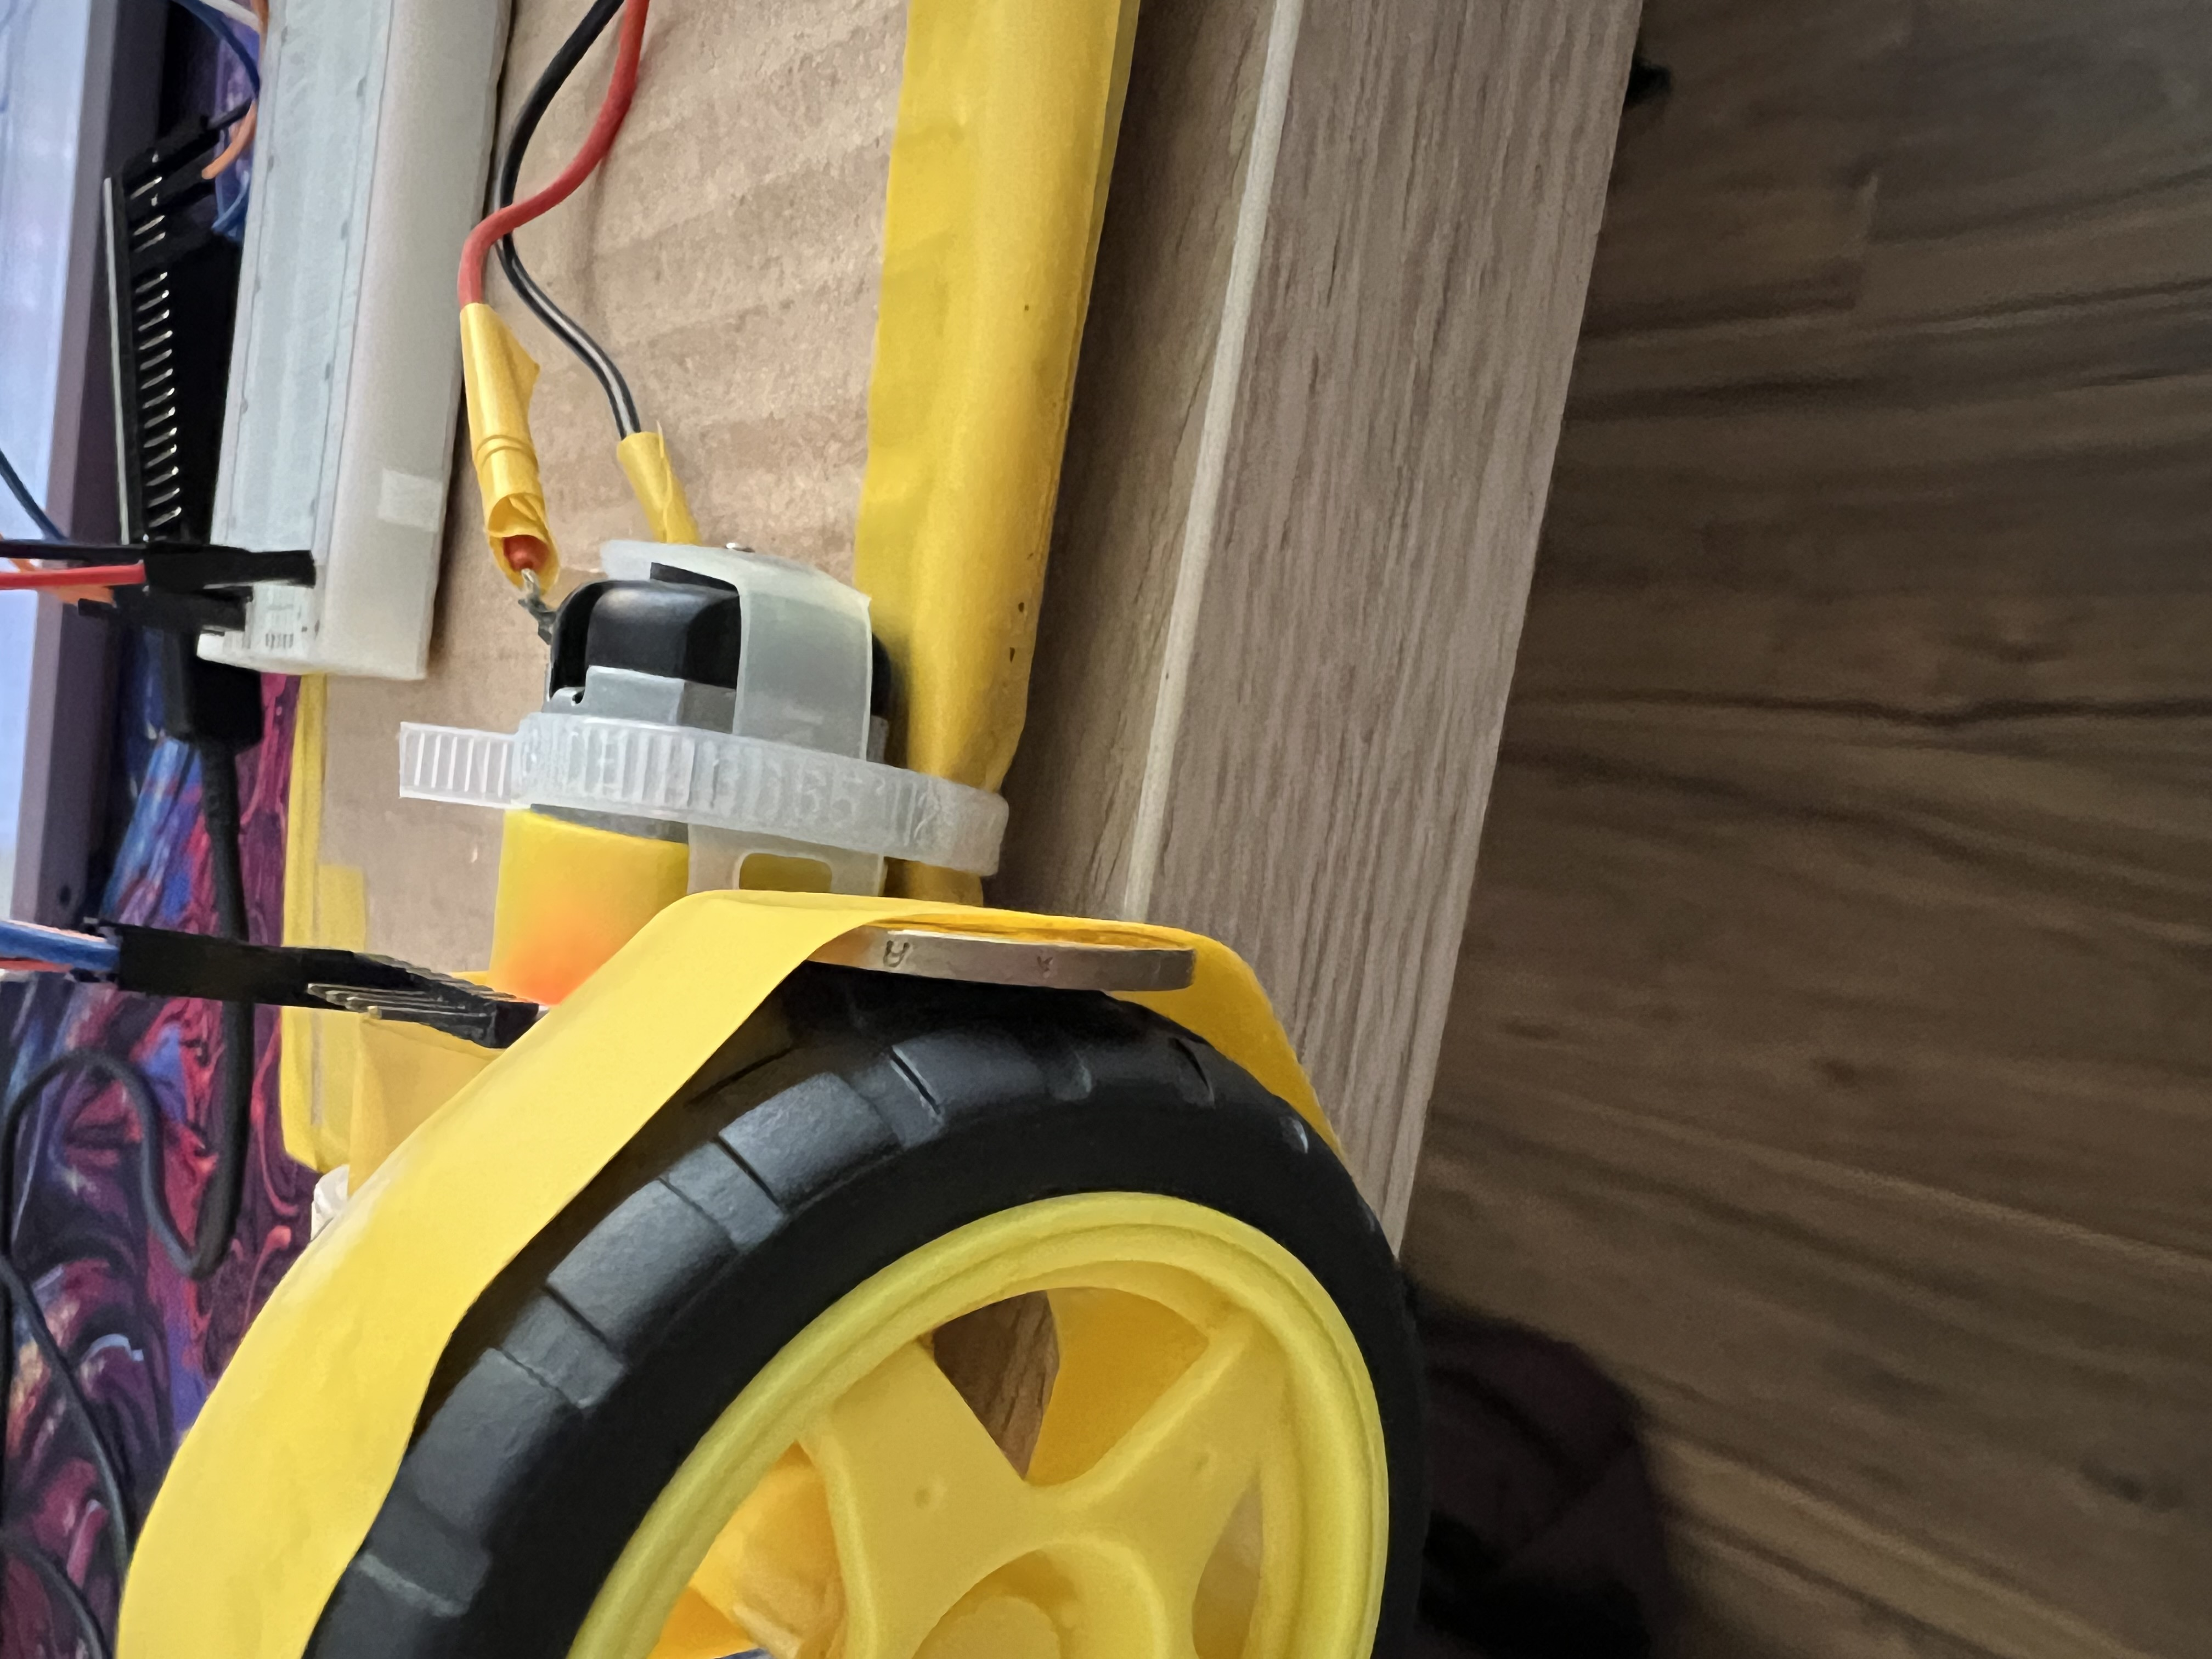
\includegraphics[width=\textwidth]{Dezechilibru.jpeg} \caption*{c) Dezechilibru} \end{minipage}
		\begin{minipage}[b]{0.3\textwidth} \centering 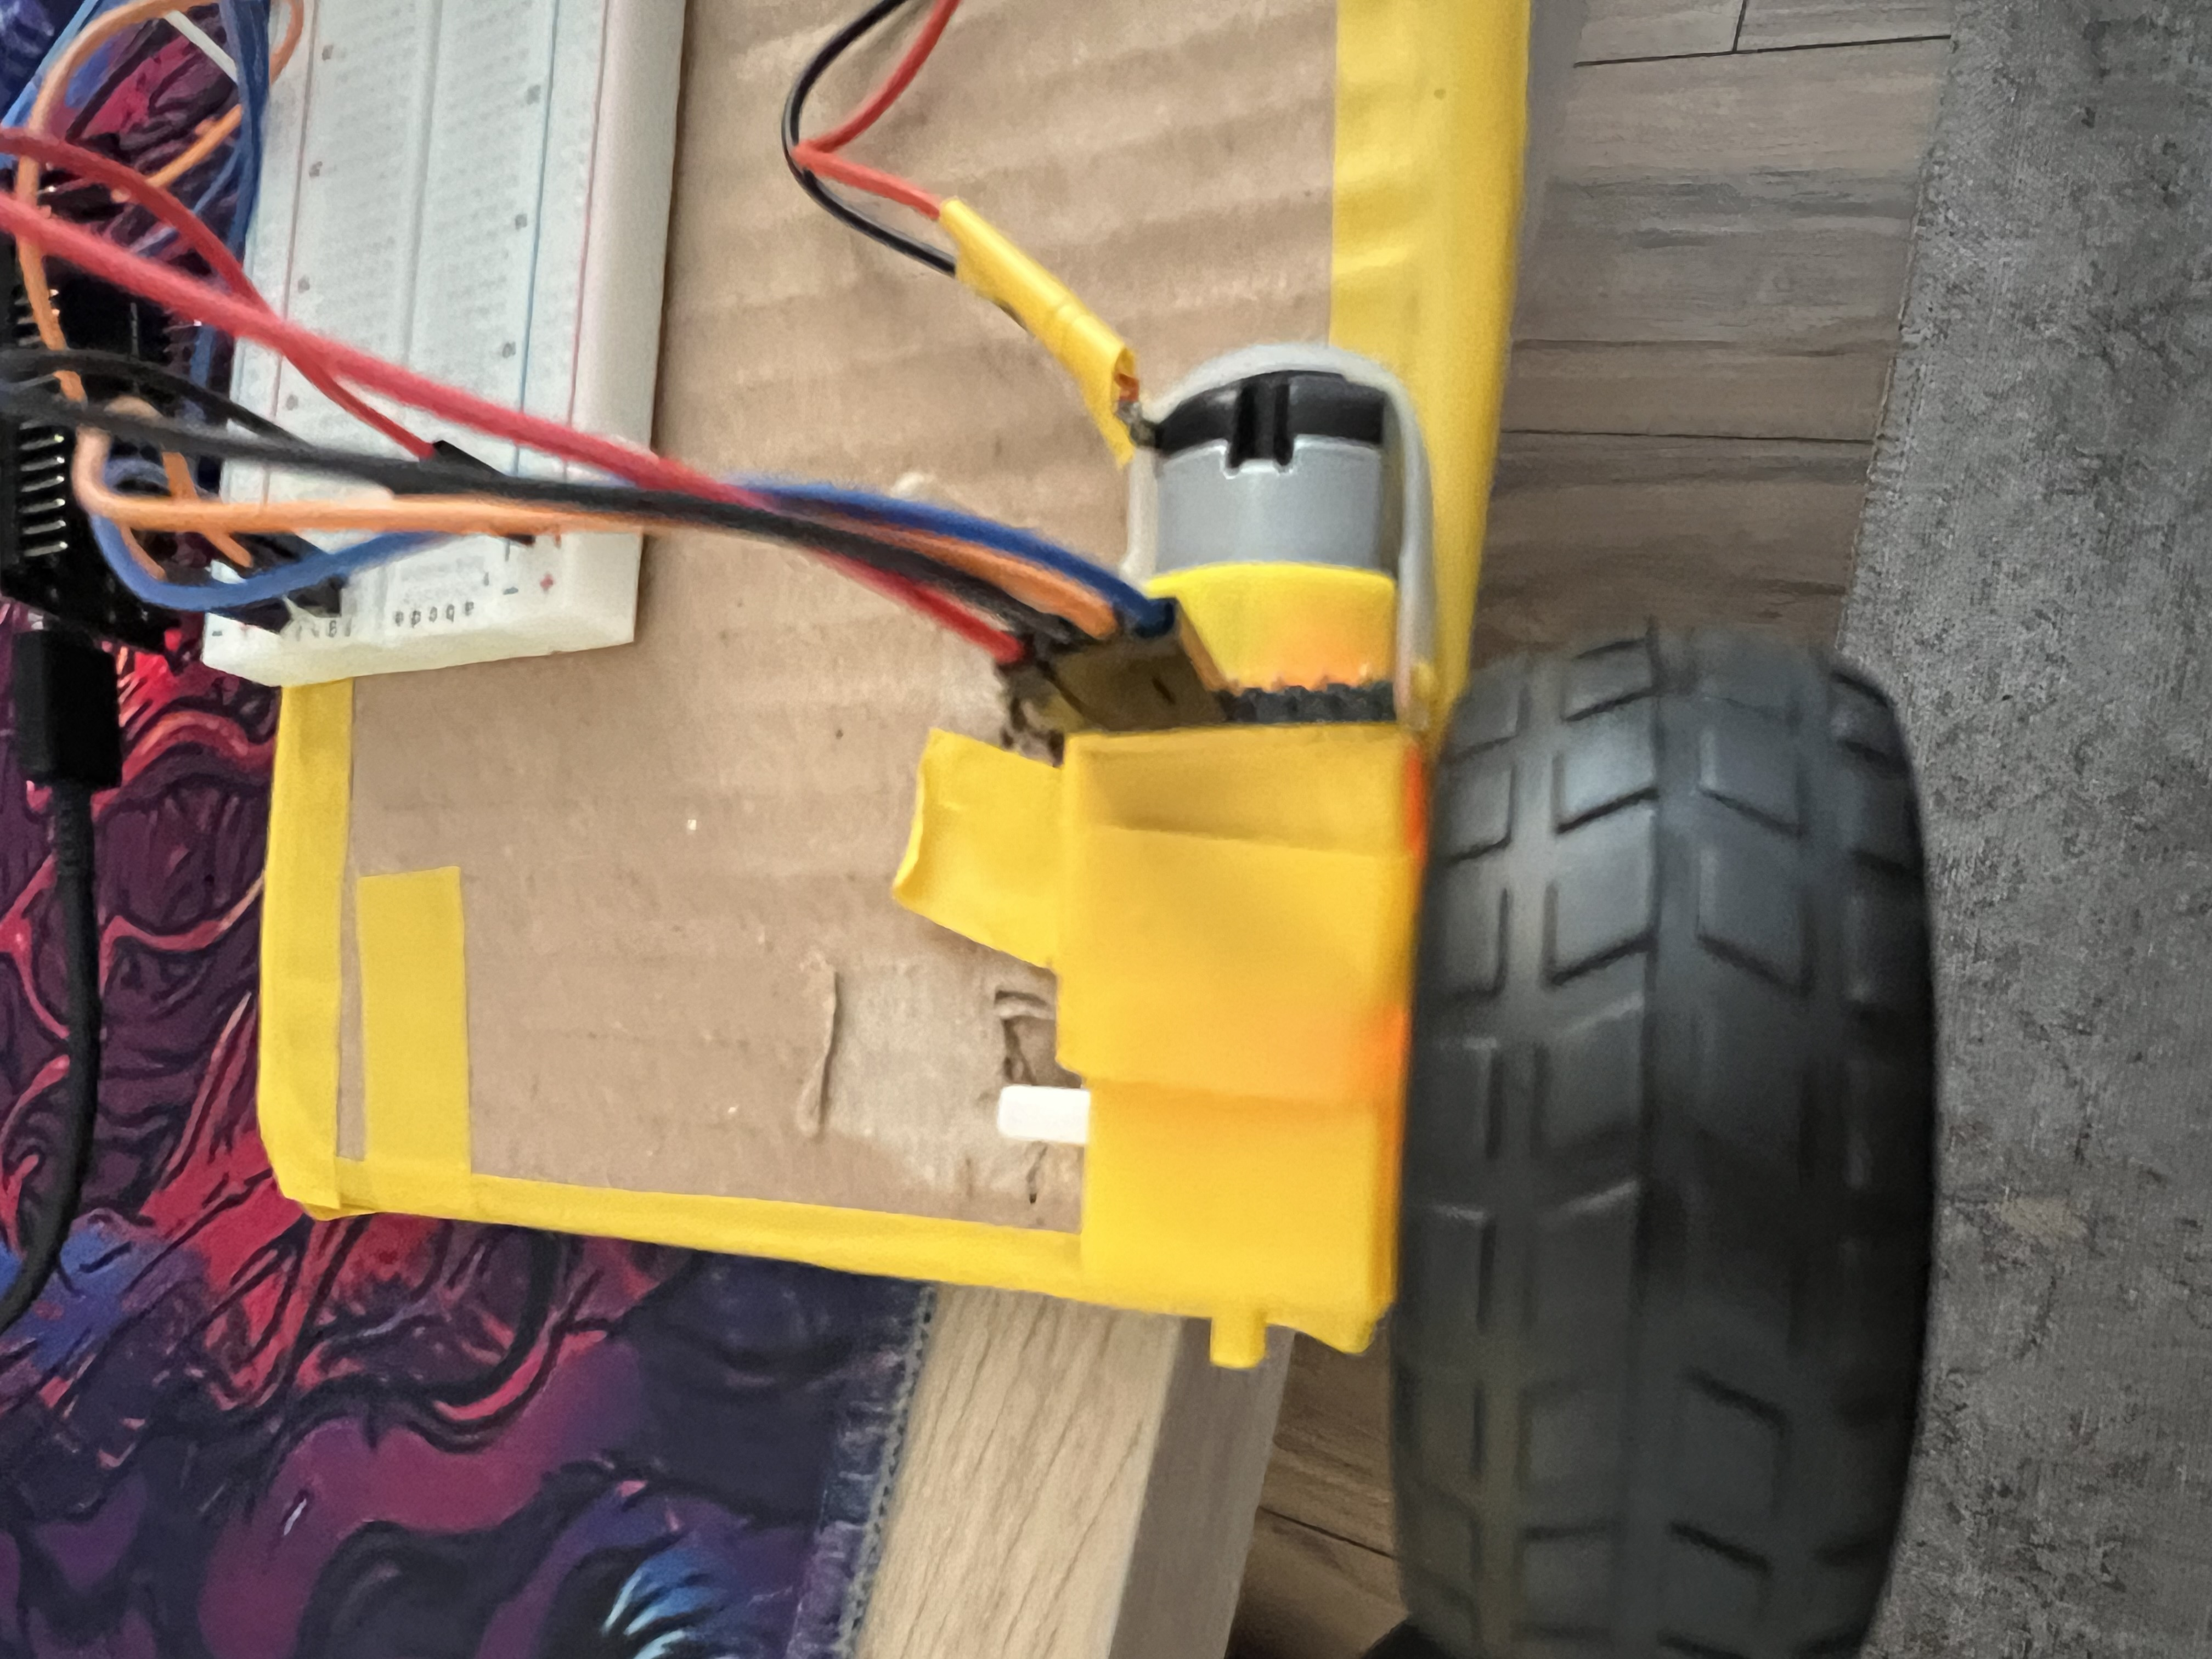
\includegraphics[width=\textwidth]{Slab_fixat.jpeg} \caption*{d) Slăbit} \end{minipage}
		\caption{Simularea fizică a scenariilor de funcționare ale motorului. Fiecare defect este indus mecanic în mod controlat, asigurând etichetarea exactă a datelor colectate.}
		\label{fig:clase_defecte}
	\end{figure}
	
	Setul de date colectate conține 538.127 de înregistrări brute, achiziția a fost realizată la o frecvență de eșantionare de 100 Hz, cu 6 viteze de PWM diferite pentru a elimina bias-ul modelului la variații de turație. Distribuția claselor este realizată astfel: clasa Repaus reprezentând 4\% din total, iar cele patru clase active sunt echilibrate, fiecare reprezentând aproximativ 24\%. Fereastra glisantă aplicată pe setul de date se rezumă la 6.727 ferestre de antrenare și 1.681 ferestre de validare.
	
	Performanța modelului CNN 1D este dependentă în mare măsură de modul în care sunt pregătite datele pentru intrare și de calitatea lor. Deoarece senzorul inerțial MPU6050 \cite{invensense:mpu6050_datasheet} furnizează măsurători brute continue, setul de date a necesitat preprocesare, aceasta fiind structurată în cinci etape.
	
	Prima etapă este segmentarea temporală prin fereastra glisantă care este descrisă la finalul Secțiunii~\ref{subsec:abordare_secventiala}.
	
	Cea de-a doua etapă este reprezentată de împărțirea setului de date. Prin împărțirea setului de date permitem evaluarea corectă a capacității de generalizare, setul final fiind împărțit în două submulțimi care păstrează strict secvența cronologică: 80\% din date au fost alocate procesului de învățare, iar restul de 20\% au fost păstrate pentru evaluarea și validarea modelului.
	
	A treia etapă este standardizarea valorilor prin normalizare, care transformă datele colectate într-o distribuție gaussiană cu media 0 și deviația standard 1. Acest pas este necesar deoarece senzorul măsoară accelerația și viteza unghiulară pe scări diferite. Pentru prevenirea situației în care o valoare are amplitudinea mai mare, astfel dominând procesul de învățare, s-a aplicat o standardizare a caracteristicilor. Parametrii de scalare au fost calculați exclusiv pe setul de antrenare, apoi utilizați pe setul de testare.
	
	În cea de-a patra etapă am aplicat o reformatare a spațiului pentru algoritmul CNN 1D. Reformatarea spațiului a fost necesară deoarece eșantioanele sunt stocate sub formă vectorială plată. Deoarece arhitectura Keras 1D CNN \cite{abadi:tensorflow} necesită ca datele să aibă o formă tridimensională specifică vectorii au fost reasamblați într-o matrice 3D de forma (număr\_eșantioane, pași\_de\_timp, număr\_caracteristici).
	
	În ultima etapă a procesării datelor am aplicat encodarea etichetelor și balansarea claselor. Etichetele explicite care descriu starea de funcționare a motorului au fost transformate. Suplimentar, deoarece clasa de repaus era subreprezentată cantitativ comparativ cu regimurile active de funcționare, s-au calculat ponderi specifice (class weights).
	
\section{Modele de Referință și Algoritmi Clasici}
	Pentru a demonstra necesitatea implementării unui model de inteligență artificială pentru detectarea anomaliilor în mod automat, am dezvoltat un algoritm clasic pentru a lua rolul de Baseline, fiind bazat pe praguri euristice. Sistemul de referință este realizat prin deviația standard și sistemul decizional prin IF-ELSE și a fost testat pe același set de date. Regulile folosite au fost stabilite pe baza deviației standard a accelerației pe axele X și Z astfel: se calculează pe fiecare fereastră dacă variațiile ambelor axe se află sub un prag minim, fereastra este clasificată drept „Repaus”, valorile care depășesc praguri succesive de amplitudine sunt asociate stărilor de defect, iar restul sunt încadrate în „Normal”.
	
	Pentru stabilirea unui punct de referință robust din perspectiva algoritmilor de învățare automată clasici am evaluat setul de date folosind următoarele metode clasice: Random Forest, Support Vector Machine cu nucleu liniar și K-Means pentru algoritmi nesupervizați.
	
	Din cauza faptului că algoritmi clasici nu au mecanisme interne pentru a interpreta seriile de timp, aceștia tratează cele 768 de valori brute ale unei ferestre ca pe niște variabile independente. Acest lucru face ca antrenarea modelelor de învățare automată clasice să aibă rezultate suboptime pe date brute. Pentru a reuși folosirea lor pe datele colectate, am introdus o etapă intermediară care extrage caracteristicile principale.
	
	Caracteristicile principale extrase, în locul datelor brute aplatizate, au fost : Media, Deviația Standard, Valoarea Root Means Square, Skewness pentru asimetria semnalului și Kurtosis pentru detectarea șocurilor mecanice, pe fiecare axă a senzorului. Prin această tehnică am redus dimensionalitatea de la 768 de valori afectate de zgomot la 30 de caracteristici dense informațional. Clasa de Repaus a necesitat o abordare diferită: deoarece semnalul ei este aproape constant, funcții matematice precum Skewness și Kurtosis generau erori de tip pierdere a preciziei. Am corectat această anomalie prin asignarea automată a valorii zero caracteristicilor de ordin superior atunci când deviația standard indică absența mișcării.
	
\section{Arhitectura Deep Learning pentru Analiza Vibrațiilor}
	
	Limitările sistemului liniar clasic, împreună cu costul computațional al preprocesării necesare algoritmilor clasici, justifică folosirea unei rețele neuronale convoluționale capabile să găsească și să extragă automat filtre pentru frecvențele ascunse în seriile de timp. În etapa de cercetare am testat trei arhitecturi convoluționale: CNN 1D, CNN 2D și CNN 3D. Arhitecturile bidimensionale și tridimensionale au o complexitate computațională mult prea mare pentru limitările fizice ale unui microcontroler, motiv pentru care am selectat arhitectura CNN 1D pentru implementarea directă pe dispozitiv. Spre deosebire de un CNN 2D, care ar fi necesitat preprocesări costisitoare precum transformarea semnalului în spectrograme, CNN 1D extrage direct corelații din datele brute.
	
	În proiectarea arhitecturii am țintit obținerea unui echilibru între capacitatea de generalizare și amprenta computațională minimă pentru a avea sens implementarea rețelei convoluționale și nu a unui algoritm de învățare automată clasic. Astfel am proiectat și implementat o rețea neuronală convoluțională unidimensională care să se muleze pe cerințe, fiind capabilă să extragă trăsăturile complexe ale seriilor de timp. Astfel arhitectura implementată primește ca intrare o matrice bidimensională de forma $(128 \times 6)$, aceasta reprezentând fereastra temporală de 128 de eșantioane pentru cele 6 axe ale senzorului. Modelul are o structură secvențială de extragere a caracteristicilor urmată de secvența de clasificare. 
	
\subsection{Extragerea Caracteristicilor}	
	
	Primul strat al rețelei neuronale este stratul Conv1D cu 16 filtre, care parcurge axa temporală, având rolul de identificare a tiparelor locale de bază precum variația bruscă de amplitudine sau frecvențe specifice de rezonanță. Apoi pentru a reduce dimensiunea spațială și a spori invarianța la mici decalaje temporale, am aplicat stratul de MaxPooling1D care înjumătățește dimensiunea temporală, prin păstrarea activărilor maxime. Acest bloc este urmat de un al doilea strat convoluțional, cu 32 de filtre, cu rolul de a combina trăsăturile de nivel inferior în reprezentări complexe definitorii pentru defecte. Urmat de un nou strat de MaxPooling1D pentru reducerea suplimentară a dimensionalității, și care pregătește datele pentru secvența de clasificare. Toate straturile convoluționale folosesc funcția non-lineară de activare ReLU. În continuare aplatizarea datelor a fost făcută cu GlobalAveragePooling1D, pentru a evita introducerea unui număr masiv de parametri prin utilizarea Flatten. Acesta calculează media fiecărei hărți de caracteristici, obținând un vector cu informație temporală de doar 32 de valori. Secțiunea de clasificare este compusă de stratul Dense complet conectat cu 32 de neuroni, urmat de stratul de ieșire cu 5 neuroni care corespund fiecărei stări de funcționare. Stratul de ieșire utilizează funcția de activare Softmax, care transformă activitatea neuronilor într-o distribuție de probabilități. Pentru a preveni overfitting-ul pe model, am folosit intercalat straturi de tip Dropout pentru dezactivarea aleatorie a unei părți de neuroni în timpul antrenamentului. \cite{abadi:tensorflow} O sinteză a topologiei rețelei și a distribuției parametrilor este prezentată în Tabelul \ref{tab:cnn_architecture}.
	
	\begin{table}[htbp]
		\centering
		\caption{Arhitectura modelului CNN 1D propus și distribuția parametrilor}
		\setlength{\tabcolsep}{4pt}
		\begin{tabular}{|l|c|c|}
			\hline
			\textbf{Layer} & \textbf{Output Shape} & \textbf{Parametri} \\ \hline
			Input & (128, 6) & 0 \\ \hline
			Conv1D (16 filtre) & (126, 16) & 304 \\ \hline
			MaxPooling1D & (63, 16) & 0 \\ \hline
			Conv1D (32 filtre) & (61, 32) & 1.568 \\ \hline
			MaxPooling1D & (30, 32) & 0 \\ \hline
			Dropout (0.2) & (30, 32) & 0 \\ \hline
			GlobalAveragePooling1D & (32) & 0 \\ \hline
			Dense (32, ReLU) & (32) & 1.056 \\ \hline
			Dropout (0.2) & (32) & 0 \\ \hline
			Dense (5, Softmax) & (5) & 165 \\ \hline
			\multicolumn{2}{|r|}{\textbf{Total Parametri:}} & \textbf{3.093} \\ \hline
		\end{tabular}
		\label{tab:cnn_architecture}
	\end{table}
	
	
	Acest design minimalist, având doar 3093 de parametri, a fost foarte eficient, în faza de antrenament fiind compilat cu funcția de cost Crossentropy și optimizatorul Adam, convergând rapid în antrenament.
	
	
\section{Optimizarea și Portarea pe Sistemul Embedded}
	
	Pentru rularea inferenței direct pe ESP32, modelul a fost compilat și integrat în PlatformIO utilizând biblioteca TensorFlowLite\_ESP32 \cite{tanaka2026tflite_esp32} un port stabilizat al framework-ului TensorFlow Lite for Microcontrollers. \cite{tensorflow:tflitemicro_github} Am aplicat o cuantizare post-antrenament (INT8) pentru conversia ponderilor Float32 în numere întregi. Aceasta a redus memoria Flash necesară la aproximativ 11,5 KB și a accelerat procesarea. De asemenea, am alocat o memorie statică de 35 KB (Tensor Arena) pentru evitarea fragmentării SRAM-ului în timpul operării. \cite{esp32_datasheet}
	
	
	Prin software am folosit sistemul de operare de timp real FreeRTOS \cite{aws:freertos}, pentru folosirea arhitecturii dual-core a ESP32. Pe Nucleul 1 am izolat achiziția I2C și execuția rețelei neuronale, sincronizate printr-o coadă de mesaje. Pe Nucleul 0 rulează procesele asincrone: serverul web și telemetria, protejate prin semafoare de excludere mutuală (Mutex).  \cite{esp32_datasheet,mathieucarbou:asynctcp, mathieucarbou:espasyncwebserver}

	